% $Id: $
\documentclass[a4paper]{article}
\usepackage[OT1]{fontenc}
\usepackage{graphicx}
\usepackage{color}
\usepackage{amsmath}
\usepackage{bbm}
\usepackage{booktabs}
\usepackage[normalem]{ulem}

\usepackage{geometry}

\usepackage[x11names]{xcolor}
\usepackage{tikz}
\usepackage{pgfplots}

\geometry{
  a4paper,
  %total={210mm, 297mm},
  %left=10mm,
  %right=10mm,
  %top=30mm,
  %bottom=20mm,
  width=160mm,
  height=210mm,
}

\renewcommand{\topfraction}{0.9}    % max fraction of floats at top
\renewcommand{\bottomfraction}{0.8} % max fraction of floats at bottom
\renewcommand{\dbltopfraction}{0.9} % fit big float above 2-col. text
\renewcommand{\textfraction}{0.07}  % allow minimal text w. figs
\renewcommand{\floatpagefraction}{0.7} % require fuller float pages
  % N.B.: floatpagefraction MUST be less than topfraction !!
\renewcommand{\dblfloatpagefraction}{0.7} % require fuller float pages

\usepackage{subfig}

\title{Fast Near-field Method for Ultrasound simulation} % the document title

\author{Jens Munk Hansen}

\def\sm{\texttt{-}}

\usepackage{hyperref}

\begin{document}

\maketitle

\thispagestyle{empty}

% Fast, uniform with known accuracy

\begin{abstract}
Bla
\end{abstract}

\begin{gather}
H_{s,l}(z;k) =
-\frac{1}{2\pi} \left(\frac{\mathrm{i}\pi}{2k}\left[\exp{(-\mathrm{i}k\sqrt{z^2+s^2+l^2})}-\exp{(-\mathrm{i}kz)}
  \right] \right.\nonumber\\
\left.-\int_{\sqrt{z^2+s^2}}^{\sqrt{z^2+s^2+l^2}}
  \arccos{\left\{\frac{s}{\sqrt{\beta^2-z^2}}\right\}}\exp{(-\mathrm{i}k\beta)}d\beta
\right.\nonumber\\
\left.-\int_{\sqrt{z^2+l^2}}^{\sqrt{z^2+s^2+l^2}}
  \arccos{\left\{\frac{l}{\sqrt{\beta^2-z^2}}\right\}}\exp{(-\mathrm{i}k\beta)}d\beta
\right)
\end{gather}

\begin{equation}
\arccos{(s/\sqrt{a^2})}=\arctan{\left(\frac{\sqrt{a^2-x^2}}{x}\right)}
\end{equation}


\begin{tikzpicture}
\begin{axis}[
    xmin=-1, xmax=2,
    ymin=-1, ymax=2,
    axis lines=center,
    axis on top=true,
    domain=0:2,
    ]

    \addplot [mark=none,draw=red,ultra thick] {sqrt(4-x*x)};
\end{axis}
\end{tikzpicture}

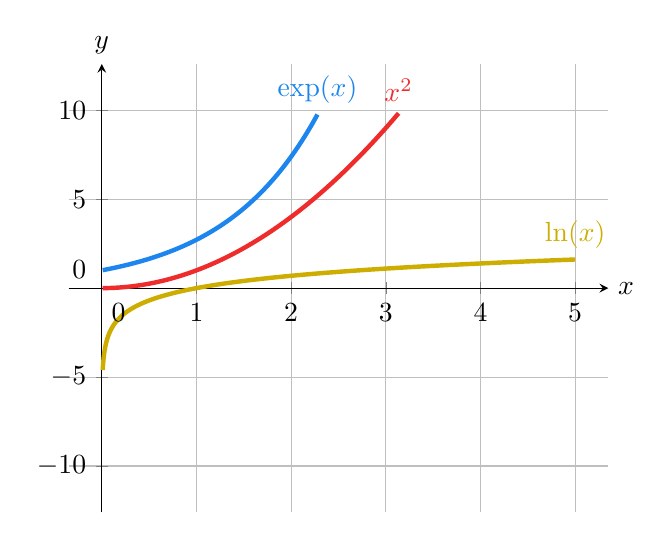
\begin{tikzpicture}
  \begin{axis}[
    grid = major,
    clip = true,
    clip mode=individual,
    restrict y to domain=-10:10,
    axis x line = middle,
    axis y line = middle,
    xlabel={$x$},
    xlabel style={at=(current axis.right of origin), anchor=west},
    ylabel={$y$},
    ylabel style={at=(current axis.above origin), anchor=south},
    domain = 0.01:5,
    xmin = 0,
    xmax = 5,
    enlarge y limits={rel=0.13},
    enlarge x limits={rel=0.07},
    ymin = -10,
    ymax = 10,
    after end axis/.code={\path (axis cs:0,0) node [anchor=north west,yshift=-0.075cm] {0} node [anchor=south east,xshift=-0.075cm] {0};},
  ]

    \addplot[color=Firebrick2,samples=100,smooth,ultra thick] {x^2} node[above,pos=1] {$x^2$};

    \addplot[color=DodgerBlue2,samples=100,smooth,ultra thick] {exp(x)} node[above,pos=1] {$\exp(x)$};

    \addplot[color=Gold3,samples=1000,smooth,ultra thick,unbounded coords=jump,no markers] {ln(x)} node[above,pos=1] {$\ln(x)$};

    %% Alternative %%

    % \addplot[color=Firebrick2,samples=100,smooth,ultra thick] {x^2} node[pos=1] (endofplotsquare) {};
    % \node [above,color=Firebrick2] at (endofplotsquare) {$x^2$};

    % \addplot[color=DodgerBlue2,samples=100,smooth,ultra thick] {exp(x)} node[pos=1] (endofplotsquare) {};
    % \node [above,color=DodgerBlue2] at (endofplotsquare) {$\exp(x)$};

    % \addplot[color=Gold3,samples=1000,smooth,ultra thick,unbounded coords=jump,no markers] {ln(x)} node[pos=1] (endofplotsquare) {};
    % \node [above,color=Gold3] at (endofplotsquare) {$\exp(x)$};
  \end{axis}
\end{tikzpicture}

\end{document}

%% Local variables:
%% TeX-master: "fnm.tex"
%% End:

% Local IspellPersDict: ~/.aspell.en.pws
